\section{Bausteinsicht}
\begin{figure}[H]
    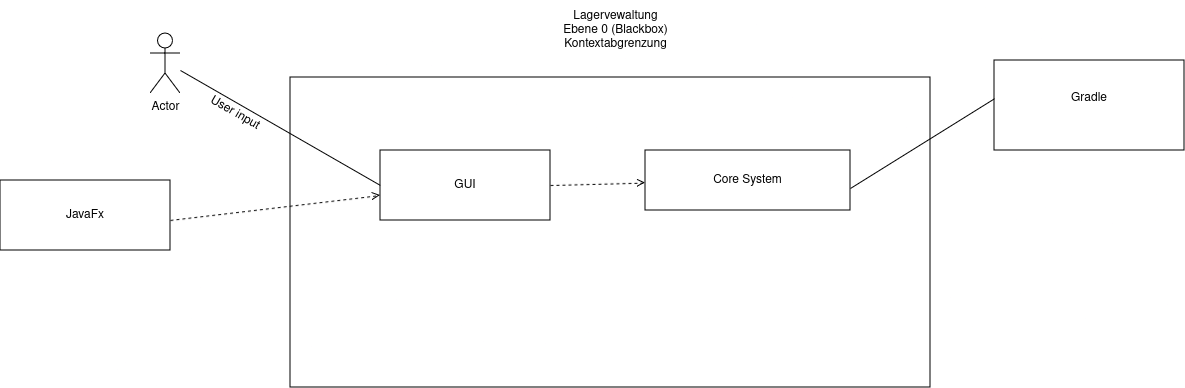
\includegraphics[width=\linewidth]{images/bausteinsicht/Ebene1_Systemuebersicht.png}
    \captionbelow{Systemübersicht}
    \label{fig:Systemuebersicht}
\end{figure}
\begin{enumerate}
    \item Begründung: Das gesamte Kernsystem mitsamt Datenhaltung, Validation und Datenmanipulation sollte dem Nutzer  nicht direkt, sondern über eine grafische Benutzer-Oberfläche angeboten werden.
    \item Enthaltene Bausteine: Die Präsentation der Daten in der Blackbox GUI, sowie das Kernsystem (Model, Service und Valiation) in der Blackbox Core System
    \item Wichtige Schnittstellen: Die Präsentationsschicht wird mithilfe von JavaFX umgesetzt. Als Build-Tool wird Gradle genutzt
\end{enumerate}
\begin{figure}[H]
    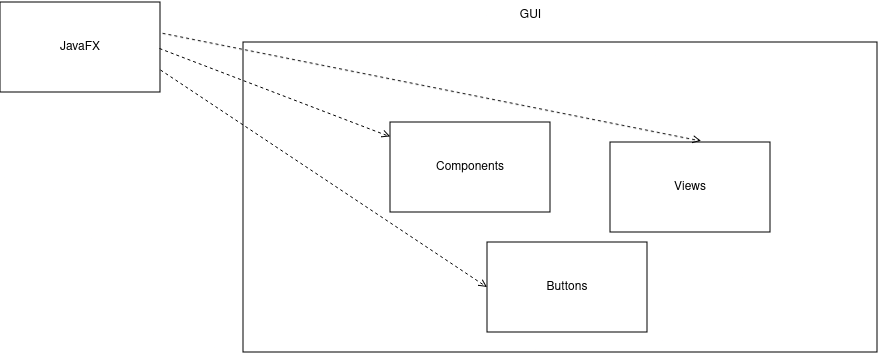
\includegraphics[width=\linewidth]{images/bausteinsicht/Ebene2_GUI.png}
    \captionbelow{GUI}
    \label{fig:GUI}
\end{figure}
\begin{enumerate}
    \item Begründung: Die GUI wurde unterteilt in Layout und Interaktionselemente
    \item Enthaltene Bausteine: Die Blackbox Views enthält Layouts von JavaFX-Elementen. In diesem Fall die Hauptansicht des Programms. Die Blackbox Buttons enthält diejenigen Interaktionselemente die diese Hauptansicht funktional beeinflussen. Die Components-Blackbox beinhaltet JavaFX-Elemente, die das Modell darstellen.
    \item Wichtige Schnittstellen: Alle Blackboxen erben von JavaFX-Klassen
\end{enumerate}
\begin{figure}[H]
    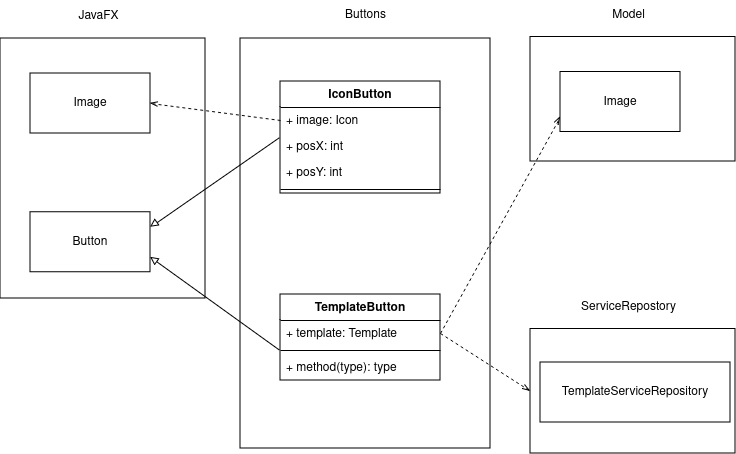
\includegraphics[width=\linewidth]{images/bausteinsicht/Ebene3_Buttons.png}
    \captionbelow{Buttons}
    \label{fig:Buttons}
\end{figure}
\begin{enumerate}
    \item Begründung: Die Buttons wurden in Buttons IconButtons, zum Umschalten der Funktionalität und TemplateButtons zum Erzeugen neuer Objekte unterteilt.
    \item Wichtige Schnittstellen: Alle Buttons erben von der JavaFX-Klasse Button
\end{enumerate}
\begin{figure}[H]
    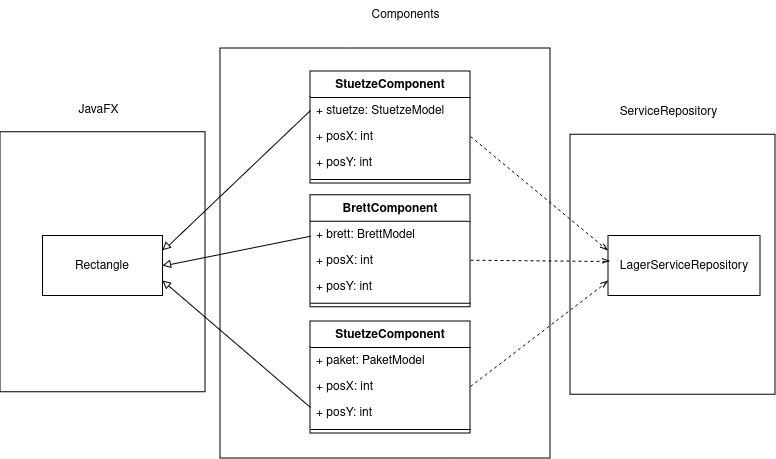
\includegraphics[width=\linewidth]{images/bausteinsicht/Ebene3_Components.png}
    \captionbelow{Components}
    \label{fig:Components}
\end{figure}
\begin{enumerate}
    \item Begründung: Die Components stellen die dem Modell zugrundeliegenden Objekte dar. Sie geben Aktionen des Nutzers an die Service Schicht weiter und hören auf ihr Modell
    \item Wichtige Schnittstellen: Alle Komponenten erben von der JavaFX-Klasse Rectangle und kommunizieren mit dem
\end{enumerate}
\begin{figure}[H]
    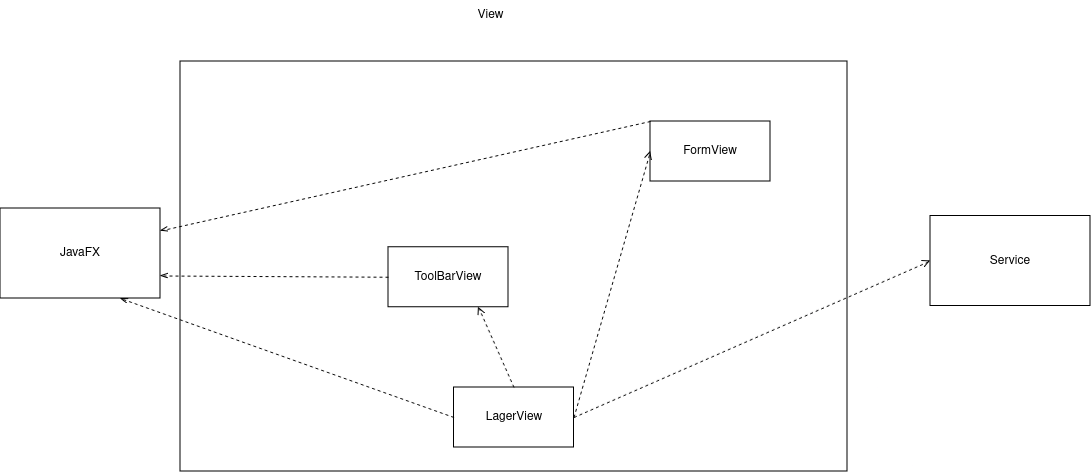
\includegraphics[width=\linewidth]{images/bausteinsicht/Ebene3_View.png}
    \captionbelow{Views}
    \label{fig:Views}
\end{figure}
\begin{enumerate}
    \item Begründung: Die Views sind alle Layouts, die auf die Scene/Stage gelegt werden. Die betten Components und Buttons ein. Views werden geschachtelt aufgebaut
    \item Wichtige Schnittstellen: JavaFX-Regions Package, Repositories zum Anzeigen des aktuellen Lagerzustands
\end{enumerate}
\begin{figure}[H]
    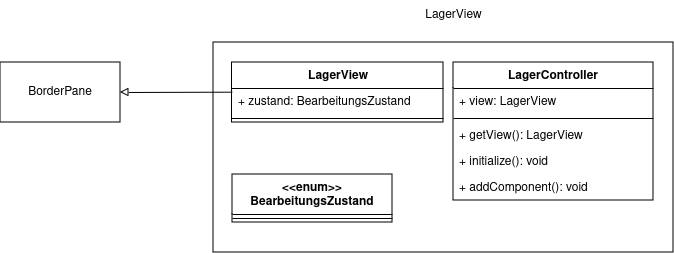
\includegraphics[width=\linewidth]{images/bausteinsicht/Ebene4_LagerView.png}
    \captionbelow{LagerView}
    \label{fig:LagerView}
\end{figure}
\begin{enumerate}
    \item Begründung: Da kein Menü geplant ist, ist der LagerView zentral. Er setzt sich aus den Komponenten und der ToolBar zusammen
    \item Wichtige Schnittstellen: LagerService um über neue Entities informiert zu werden
\end{enumerate}
\begin{figure}[H]
    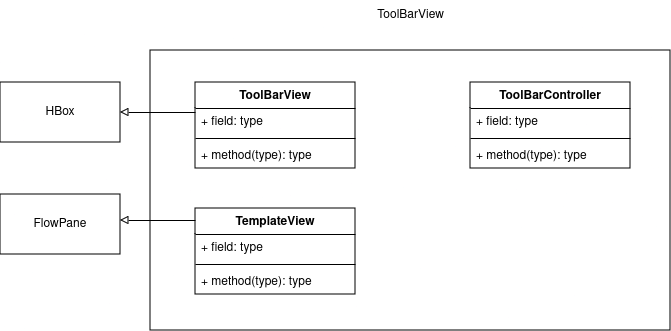
\includegraphics[width=\linewidth]{images/bausteinsicht/Ebene4_ToolBarView.png}
    \captionbelow{ToolBarView}
    \label{fig:ToolBarView}
\end{figure}
\begin{enumerate}
    \item Begründung: Die ToolBar bietet alle Buttons an. Sie schaltet zwischen den Modi des Systems um.
    \item Wichtige Schnittstellen: LagerView
\end{enumerate}
\begin{figure}[H]
    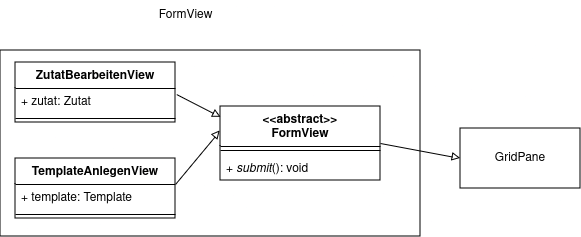
\includegraphics[width=\linewidth]{images/bausteinsicht/Ebene4_FormView.png}
    \captionbelow{FormView}
    \label{fig:FormView}
\end{figure}
\begin{enumerate}
    \item Begründung: Die FormView ist gedacht zum Anlegen neuer Zutaten und Templates. Sie spricht direkt mit den jeweiligen Service-Klassen um ihr eigenes Modell anlegen zu lassen
    \item Wichtige Schnittstellen: ZutatService und TemplateService
\end{enumerate}
\begin{figure}[H]
    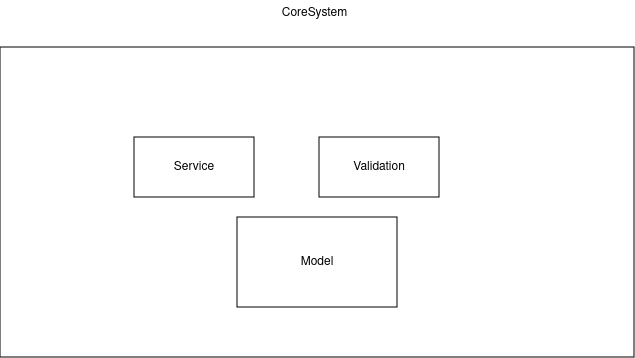
\includegraphics[width=\linewidth]{images/bausteinsicht/Ebene2_Core.png}
    \captionbelow{Core}
    \label{fig:Core}
\end{figure}
\begin{enumerate}
    \item Begründung: Das Core-System umfasst die Modellwelt und die sie ändernde (ServiceRepository) und überprüfende Schicht (Validator)
    \item Wichtige Schnittstellen: Service-Klassen als Schnittstelle zur GUI, Modell-Struktur als Grundlage der Datenhaltung
\end{enumerate}
\begin{figure}[H]
    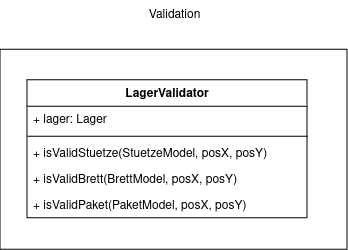
\includegraphics[width=\linewidth]{images/bausteinsicht/Ebene3_Validation.png}
    \captionbelow{Validation}
    \label{fig:Validation}
\end{figure}
\begin{enumerate}
    \item Begründung: Validierung sollte optional von der Modellschicht sein, damit man sie freier nutzen kann. Validierung ist in dieser Anwendung zwingend erforderlich um valide Aktionen des Nutzers zu bestimmen
    \item Wichtige Schnittstellen: ServiceRepository um auf aktuellen Zustand des Lagers zugreifen zu können
\end{enumerate}
\begin{figure}[H]
    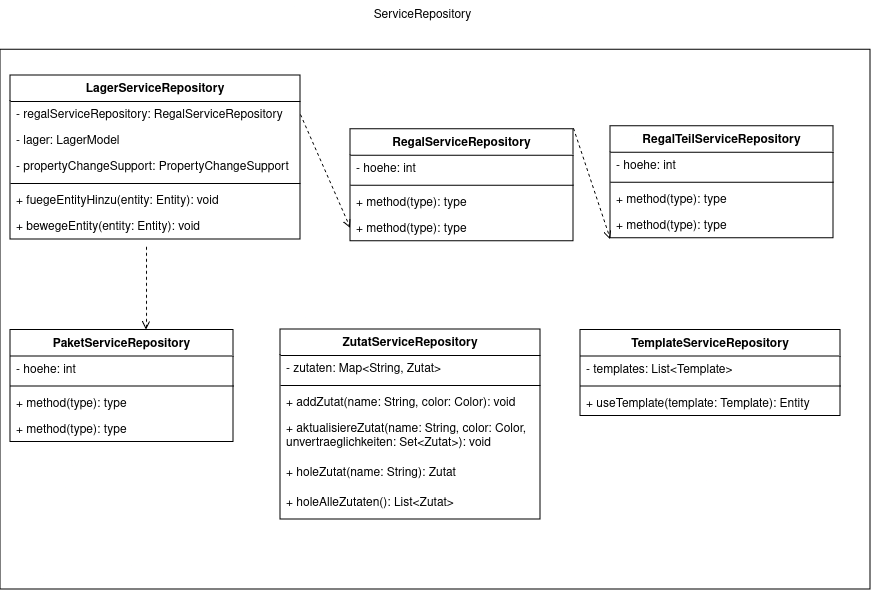
\includegraphics[width=\linewidth]{images/bausteinsicht/Ebene3_ServiceRepository.png}
    \captionbelow{ServiceRepository}
    \label{fig:ServiceRepository}
\end{figure}
\begin{enumerate}
    \item Begründung: Das ServiceRepository ist die Haltung der Daten und ihrer Manipulation zuständig. Ein separates Repository ist aufgrund der gerinen Dateimenge nicht notwendig, die Objekte werden in Dateien gespeichert.
    \item Wichtige Schnittstellen: GUI, um Aktionen des Nutzers zu empfangen
\end{enumerate}
\begin{figure}[H]
    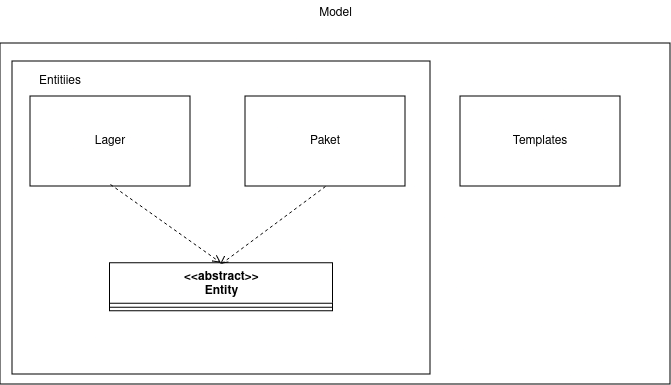
\includegraphics[width=\linewidth]{images/bausteinsicht/Ebene3_Model.png}
    \captionbelow{Model}
    \label{fig:Model}
\end{figure}
\begin{enumerate}
    \item Begründung: Das Modell ist in zwei Teile aufgeteilt. Templates sind wiederverwendbar, aber nicht notwendig um das Modell zu nutzen. Entities können standardisiert erstellt werden und zusammen verwaltet werden.
    \item Wichtige Schnittstellen: Entity-Package ist zentral
\end{enumerate}
\begin{figure}[H]
    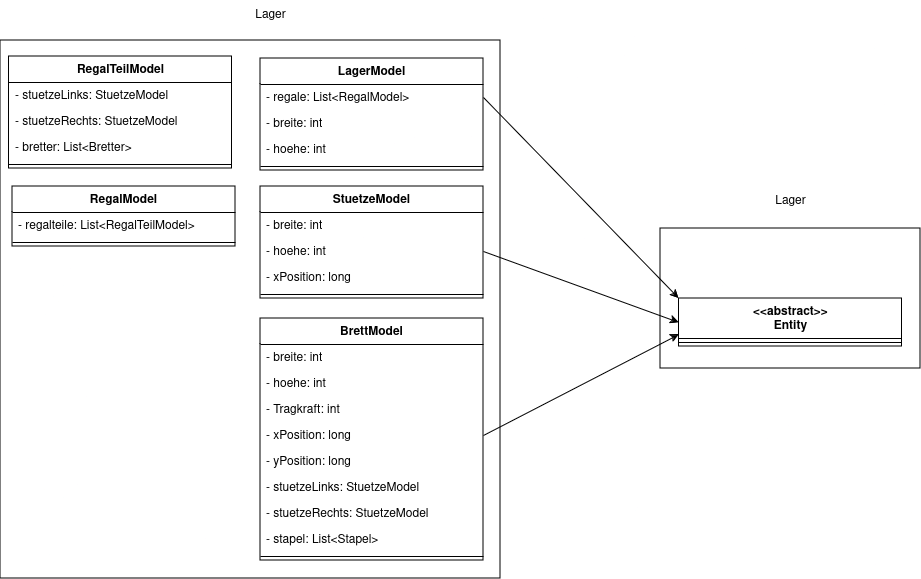
\includegraphics[width=\linewidth]{images/bausteinsicht/Ebene4_Lager.png}
    \captionbelow{Lager}
    \label{fig:Lager}
\end{figure}
\begin{enumerate}
    \item Begründung: Die Teile des Lagers, die in der GUI auftauchen erben von Entity. Separate Klassen, die nur im internen Aufbau des Lagers wichtig sind, erben nicht davon und können dementsprechend nicht über Templates erstellt werden
\end{enumerate}
\begin{figure}[H]
    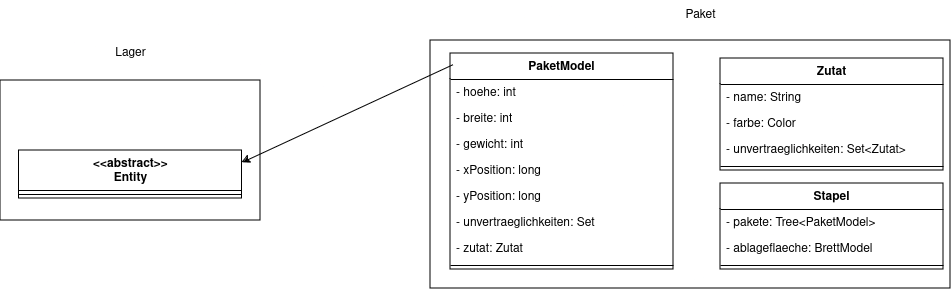
\includegraphics[width=\linewidth]{images/bausteinsicht/Ebene4_Paket.png}
    \captionbelow{Paket}
    \label{fig:Paket}
\end{figure}
\begin{enumerate}
    \item Begründung: Das PaketModel ist wieder ein Entity, die Zutaten werden separat verwaltet.
\end{enumerate}
\begin{figure}[H]
    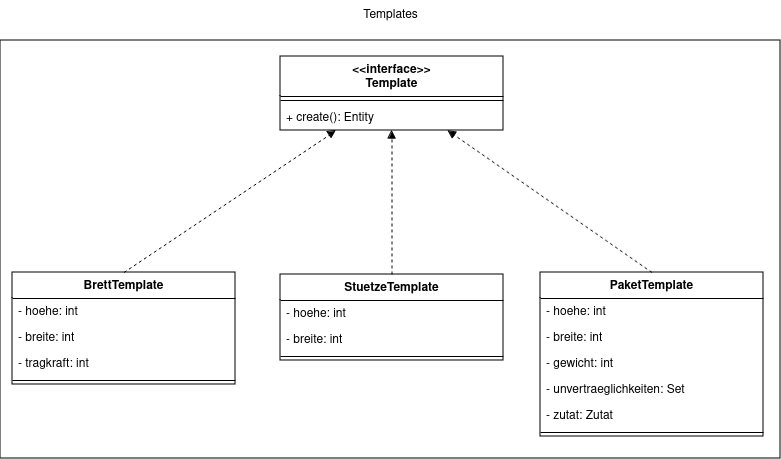
\includegraphics[width=\linewidth]{images/bausteinsicht/Ebene4_Template.png}
    \captionbelow{Template}
    \label{fig:Template}
\end{figure}
\begin{enumerate}
    \item Begründung: Templates werden separat von den Entities gehalten um über die GUI einfach dargestellt zu werden.
    \item Wichtige Schnittstellen: TemplateButtons
\end{enumerate}